\chapter{Antecedentes}
\label{chap:antecedentes}

\drop{E}n  este  capítulo  se  revisarán los  conceptos  y  cuestiones
básicas  que sentarán  las bases  para comprender  el alcance  de este
\acs{TFG} y el especial contexto en el que éste se enmarca. Para ello,
ofreceremos  una serie  de definiciones  esenciales y  analizaremos la
situación actual de los sistemas de seguridad, desde el punto de vista
de las  soluciones comerciales que  existen en  el mercado y  desde la
perspectiva  de   las  previsiones   de  algunos  directores   de  las
principales compañías del mercado.

\section{Conceptos básicos dentro de un sistema de seguridad}
El sector de  la seguridad, y más concretamente en  el de los \acf{SES}, manejan  una  serie  de  conceptos  cuyo
significado  ha  de  ser  establecido  previamente  para  que  podamos
comprender cómo se ha de abordar  la creación, comparación o  gestión de
cualquier sistema de  seguridad.  Cuesta trabajo definir  un sistema o
una  aplicación en  el  área  de la  seguridad  sin  los conceptos  de
\textit{estado},   \textit{partición},  \textit{tipos   de  zona},   o
\textit{grado}. Las siguientes subsecciones analizarán con más detalle
estos conceptos.

\subsection{Grado de seguridad de los sistemas}

En cuanto a legislación en materia  de seguridad, España es uno de los
países  de  la  Unión  Europea  que más  normas  aplica  con  carácter
obligatorio.  Esto  se  ha  hecho  con  el  fin  de  homogeneizar  las
diferentes  normativas  existentes  en  la actualidad  en  los  países
miembros de  la comunidad  y para  que las  condiciones técnicas  y de
seguridad sean  equivalentes a las exigidas  en cada uno de  ellos. De
esta forma, en nuestro país, se ha considerado necesario utilizar normas
europeas aprobadas a nivel comunitario y destinadas de forma expresa a
regular las  características técnicas  de los elementos  que conforman
los sistemas de alarmas o \acs{SES}~\cite{BOE}.

«Para ello resultan de aplicación las Normas UNE-EN 50130, 50131, 50132, 50133, 50136 y la Norma UNE CLC/TS 50398, dedicadas a establecer los requisitos generales de los sistemas de alarma, los grados de seguridad, las clases ambientales, el diseño de los sistemas, su planificación, funcionamiento y mantenimiento»~\cite{BOE}.

Quizás,  de   todas  las  normas  anteriormente   mencionadas,  la  más
importante sea la norma UNE-EN  50131-1 que establece cuatro grados de
seguridad en función del riesgo. Establecido en la Orden INT/316/2011,
del 1 de febrero, sobre funcionamiento de los sistemas de alarma en el
ámbito  de  la seguridad  privada.  Esta  orden ministerial  establece
además  la  aplicación  de   los  grados  de  seguridad  anteriormente
comentados en virtud de la naturaleza y característica del lugar en el
que se va a efectuar la instalación y de la obligación, o no, de estar
conectados a una central de alarmas o centro de control~\cite{BOE}.


\begin{quote}
{\itshape
\begin{itemize}
\item \textbf{Grado 1}, o de bajo riesgo, para sistemas de seguridad dotados de señalización acústica, que no se vayan a conectar a una central de
alarmas o centro de control.
\item \textbf{Grado 2}, de riesgo bajo a medio, dedicado a viviendas y pequeños establecimientos,
comercios e industrias en general, que pretendan conectarse a una central de alarmas o,
en su caso, a un centro de control.
\item \textbf{Grado 3}, de riesgo medio/alto, destinado a establecimientos obligados a disponer
de medidas de seguridad, así como otras instalaciones comerciales o industriales a las
que por su actividad u otras circunstancias se les exija disponer de conexión a central de
alarmas o, en su caso, a un centro de control.
\item \textbf{Grado 4}, considerado de alto riesgo, reservado a las denominadas infraestructuras
críticas, instalaciones militares, establecimientos que almacenen material explosivo
reglamentado, y empresas de seguridad de depósito de efectivo, valores, metales
preciosos, materias peligrosas o explosivos, requeridas, o no, de conexión con central de
alarmas o, en su caso, a centros de control.
\end{itemize}
}
\nopagebreak
\par\nointerlineskip\noindent\hfill Orden INT/316/2011~\cite{BOE}
\end{quote}

Una observación curiosa dentro de la normativa aparece en el « Artículo 3. Aprobación de material » exactamente en el punto cuatro, que viene a decir básicamente: ``Una cadena es tan fuerte como su eslabón más débil.'' Veamos a que nos referimos:

\begin{figure}[!h]
\centering
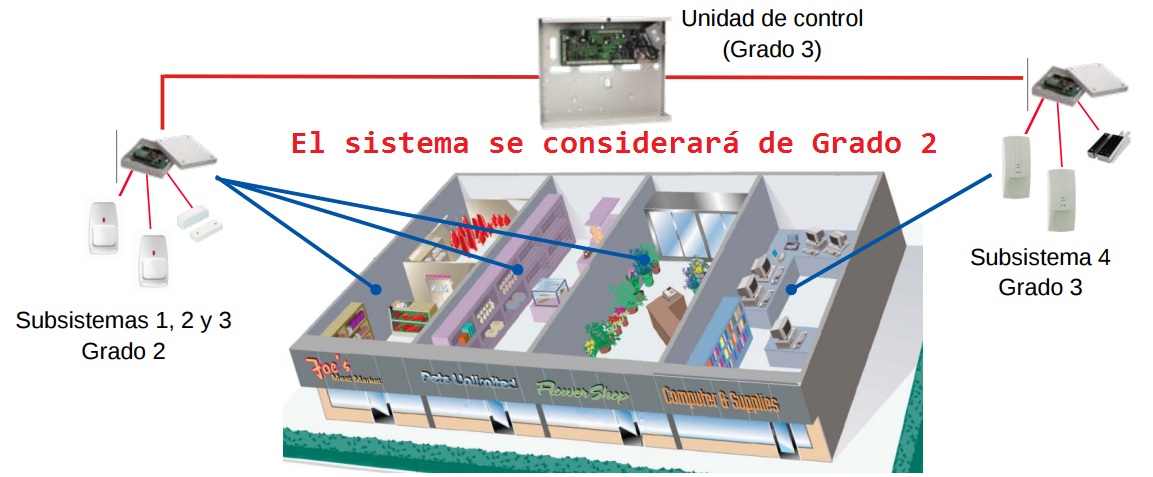
\includegraphics[width=1\textwidth]{/system_degree.png}
\caption{Aprobación de Grado de una Instalación de seguridad}
\label{fig:system_degree}
\end{figure}

\begin{itemize}
\item «En caso de que un sistema de alarma se divida en subsistemas claramente definidos, será posible que dicho sistema incorpore componentes de distintos grados en cada subsistema».
\item «El grado correspondiente al subsistema será equivalente al grado más bajo aplicable a uno de sus componentes».
\item «El grado correspondiente al sistema será equivalente al grado más bajo aplicable a sus subsistemas».
\end{itemize}

Podemos concluir de lo expuesto anteriormente que a una instalación de seguridad se le adjudicará el grado correspondiente al elemento de menor graduación que la integre (ver Figura~\ref{fig:system_degree})~\cite{BOE}.

\subsection{Estados}
Cuando hablamos de estados en un \acf{SES} estos pueden ser lógicos o físicos ya sean de un sensor o de una de las controladoras que componen el sistema. Aunque es bastante frecuente que la terminología de estos se acabe mezclando y se usen indistintamente en ambos. Por ejemplo:

\subsubsection{Estados Físicos}
\label{sec:estados-fisicos}

Si nos  referimos a los  estados físicos  de un sensor  de \acf{GIII}
como  pueda  ser  el  volumétrico  DT7550  de  doble  tecnología  (ver
Cuadro~\ref{tab:dt7550-overview}), podemos  identificar los siguientes
estados:

\begin{itemize}
\item \textbf{Abierto:} Es un estado de detección comprendido dentro del funcionamiento normal del dispositivo. Dependiendo del fabricante hace referencia a una lectura de 2 k$\Omega$ por parte de la central o controladora que esté supervisando el detector. Su homólogo en estados lógicos sería \textbf{Alarma} o cualquier otro sinónimo elegido por el fabricante que indique detección.
\item \textbf{Cerrado:} Es el estado que más gusta a los operadores de los sistemas puesto que indica que todo es correcto y va bien. Dependiendo del fabricante hace referencia a una lectura de 1 k$\Omega$ por parte de la central o controladora que esté supervisando el detector. Su homólogo en estados lógicos sería \textbf{Reposo} o cualquier otro sinónimo elegido por el fabricante que indique la ausencia de detección.
\item \textbf{Tamper:} Es un estado de detección anómalo, indicativo de sabotaje o mal funcionamiento en el dispositivo. Dependiendo del fabricante hace referencia a una lectura de $\infty$ $\Omega$ o 4.7 k$\Omega$ por parte de la central o controladora que esté supervisando el detector. Su homólogo en estados lógicos sería \textbf{Sabotaje} o cualquier otro sinónimo elegido por el fabricante que indique manipulación o mal funcionamiento.
\item \textbf{Cortocircuito:} Es un estado de detección anómalo, indicativo de sabotaje o mal funcionamiento en el cableado del dispositivo. Dependiendo del fabricante hace referencia a una lectura de 0 $\Omega$ o valores extremadamente bajos por parte de la central o controladora que esté supervisando el detector. Su homólogo en estados lógicos sería \textbf{Sabotaje} o cualquier otro sinónimo elegido por el fabricante que indique manipulación o mal funcionamiento.
\item  \textbf{Enmascaramiento:}  Es  un   estado  que  cumplimenta  a
  aquellos  dispositivos  que  detectan, empleando  doble  tecnología,
  \acf{MW} y \acf{PIR} y  normalmente exclusivo de aquellos detectores
  que cumplen con \acs{GIII}. Este  es un estado de detección anómalo,
  indicativo  de sabotaje  o  de  mala configuración  y  ajuste en  la
  sensibilidad   del  detector.   Dependiendo   del  fabricante   hace
  referencia a  una lectura de 3  k$\Omega$, por parte de  la central o
  controladora  que  esté supervisando  el  detector.  Su homólogo  en
  estados  lógicos  sería  \textbf{Enmascaramiento} o  cualquier  otro
  sinónimo elegido  por el fabricante  que indique manipulación  o mal
  funcionamiento.
\end{itemize}

\begin{table}[hp]
  \centering
  \centering
  \caption{Características Técnicas Detector DT7550 \cite{HoneywellDT7550}}
  \label{tab:dt7550-overview}
  \zebrarows{1}
  {\small
  
\begin{tabular}{p{0.48\textwidth}p{0.48\textwidth}}
  \hline
\textbf{Característica} & \textbf{Valor} \\
\hline
Range & 15 x 18 m\\
PIR Fields of View & 22 long range edges, 12 intermiate edges, 6 lower edges, 4 look-down edges \\
Sensitivity & Low (Pulse Count 2): 3-4 steps / High (Pulse Count 1): 2-3 steps\\
Frecuencies & 24.200 GHz (k Band) \\
Mounting Height & 2.3 m \\
Power Requirements & 9-15VDC - 25 mA \\
Anti-masking technology & Microwave \\
RFI Immunity & 30 V/m, 10 MHz – 1000 MHz \\
PIR White Light Immunity & 6 500 Lux \\
Operating Temperature & -10$^{\circ}$C to +55$^{\circ}$C \\
Relative Humidity & 5\% – 95 \% relative humidity (non-condensing) \\
\acs{EOL} Alarm Resistor & 1k$\Omega$, 2.2k$\Omega$, 4.7k$\Omega$ and 5.6k$\Omega$ ; default = 1k$\Omega$ \\
\acs{EOL} Tamper Resistor & 1k$\Omega$, 2.2k$\Omega$, 4.7k$\Omega$ and 5.6k$\Omega$ ; default = 1k$\Omega$ \\
\acs{EOL} Mask Resistor & 2.2k$\Omega$, 3k$\Omega$; default = 1k$\Omega$ \\ 
\hline
\end{tabular}

  }
\end{table}

\subsubsection{Estados Lógicos}

Los estados lógicos son aquellos que puedan representar:

\begin{enumerate}
  \item Un estado físico del detector (ver \hyperref[sec:estados-fisicos]{\textit{Estados Físicos}}) en el sistema en un momento concreto como: \textbf{Alarma}, \textbf{Reposo}, \textbf{Sabotaje} y \textbf{Enmascaramiento}.
  \item Un modo de funcionamiento del detector que no corresponde exactamente con un estado físico pero aporta valor en la gestión del sistema de seguridad.
\end{enumerate}

 Aunque pueden existir tantos estados lógicos como los fabricantes deseen o encuentren apropiados para sus \acs{SES}, entre los más empleados podemos encontrar:

 \begin{itemize}
 \item \textbf{Omitido:} Este es uno de los estados más importantes de cara al correcto funcionamiento de cualquier \acs{SES} o plataforma integradora de subsistemas de seguridad. Sin este estado los sistemas serían inoperables ante una avería. Se emplea básicamente para decirle al sistema que ignore cualquier estado que provenga del detector o grupo de detectores y que no actúe siguiendo el protocolo establecido.
 \item \textbf{Alarma Reconocida:} Como su nombre indica, este estado representa una alarma reconocida por el operador que no se quiere seguir recibiendo y no se quiere omitir. Dependiendo del fabricante y del sistema, este estado puede no existir explícitamente (varias centrales del mercado como la Galaxy Flex \cite{Honeywell} carecen de este estado) y puede variar su funcionamiento. Por ejemplo: en plataformas como Desico, no se registran nuevos eventos u estados hasta que el  detector no está en reposo y en otras desaparece este estado ante cualquier cambio físico diferente al anterior (el que provoca el estado).
 \end{itemize}

\subsection{Particiones y Zonas}
\label{sub:particiones_zonas}

En los \acs{SES} las particiones o áreas, como también son conocidas, constituyen una herramienta fundamental para la operabilidad de los mismos. Por una parte permiten hacer agrupaciones de los detectores por regiones operativas o por su tipo (véase Figura~\ref{fig:galaxy_partition}), por otra parte, permiten al operador dar órdenes o poner en un estado determinado a todos los elementos pertenecientes a la partición.

\begin{figure}[!h]
\centering
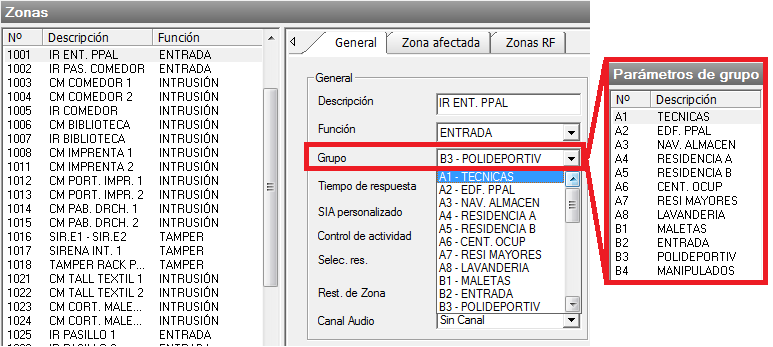
\includegraphics[width=1\textwidth]{/galaxy_partition.png}
\caption{Asignación de una zona a un grupo}
\label{fig:galaxy_partition}
\end{figure}

Una zona, sin embargo, no es  más que la representación de un detector
en un  sistema y  dependiendo de  su tipo,  el modo  de funcionamiento
dentro del sistema de seguridad variará.

A continuación se  explican algunos de los tipos de  zonas más comunes
en los \acs{SES}. Hay que destacar que hay tantos tipos de zonas como
nuevos modos de  funcionamiento pueda encontrar un  fabricante para un
detector, pero en esencia, los que  aquí se comentan, se encuentran en
la mayoría de sistemas comerciales con estos nombres u otros.

\begin{itemize}
\item \textbf{Intrusión:} Es el tipo de zona mayoritariamente empleada en todas las instalaciones. Describe un funcionamiento estándar de alarma cuando la partición a la que pertenece se encuentra armada y hay una detección. En caso de estar su partición desarmada representa los diferentes estados físicos del detector en el \acs{SES}, sin gestionarse ninguna alarma a menos  que se presente un estado lógico de sabotaje.
\item \textbf{24 Horas:} Como su nombre  indica este tipo de zona hace
  que   el   detector   se   gestione   en   el   \acs{SES}   siempre,
  independientemente de si la partición a la que pertenece el detector
  se encuentra  armada o  desarmada. Este tipo  de gestión  se realiza
  para supervisar  detectores que protegen las  controladoras, placas
  del  sistema, o  señales  críticas  como puedan  ser  una alarma  de
  incendio, una fuga de gas, fallo de refrigeración, etc.
\item \textbf{Entrada/Salida:} Es el tipo de función a asignar a todos aquellos detectores que se encuentran cercanos al acceso o salida principal del área a proteger. Este tipo de zona omite cualquier detección durante un periodo de tiempo establecido, en la partición a la que pertenece, para la entrada o salida del recinto. De esta forma se permite al operador o usuario del sistema, entrar o salir del recinto para armar o desarmar sin emitir ninguna alarma,  dentro del periodo de tiempo establecido.
\item \textbf{Atraco silencioso:} Es la función que por excelencia se le asigna a los pulsadores de atraco. Al igual que el tipo de zona 24 horas, el detector está siendo siempre gestionado por el \acs{SES}, independientemente de que su partición se encuentre armada o desarmada. La particularidad que define a este tipo de zona es que jamás emite ningún tipo de aviso sonoro, con el fin de no disuadir al atracador o agresor, enviando una alerta de atraco a la \acf{CRA} en caso de existir o a otra persona responsable de la supervisión del sistema.
\item \textbf{Llave:} Esta función suele reservarse para el armado o desarmado de una partición a través de un contacto como pueda ser un relé activado por un subsistema o por otra partición. Normalmente y dependiendo del fabricante solo se permite que exista una zona de este tipo por partición para evitar comportamientos indeseados.
\end{itemize}

\section{Hardware de bajo coste}
\label{chap:low-cost-hw}

A día de hoy el mercado se encuentra saturado de versiones comerciales, más o menos seguras, de sistemas de seguridad que podrían entrar dentro de la gama de bajo coste (ver Figura~\ref{fig:lc_alarm}). La mayoría de estos sistemas están concebidos para entornos domésticos, no cumplen con \acs{GII} y son extremadamente vulnerables ante inhibidores de frecuencias e interferencias electromagnéticas producidas por motores eléctricos, fluorescentes y otras clases de dispositivos. Sin embargo, a pesar de que existen una gran variedad de fabricantes que han optado por buscar su nicho de mercado ofreciendo precios bajos, a diferencia del sector domótico, a día de hoy sigue sin existir explícitamente, una plataforma concebida para soportar detectores de \acs{GII} y \acs{GIII} que sea completamente de código y hardware abierto.

\begin{figure}[!h]
\centering
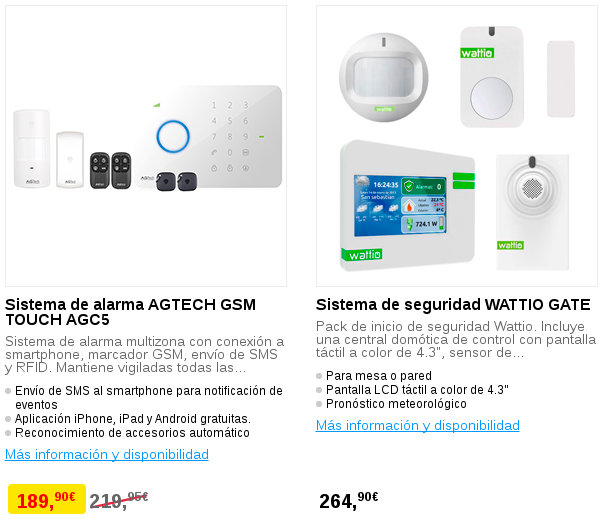
\includegraphics[width=0.8\textwidth]{/lc_alarm.png}
\caption{Productos a la venta en Leroy Merlin~\cite{Leroy}}
\label{fig:lc_alarm}
\end{figure}

Esta misma situación, pero en el sector educativo, ha sido la principal causa de la aparición de las plataformas Arduino y Raspberry Pi en el año 2005 y 2012 respectivamente. A continuación y antes de adentrarnos más en las soluciones profesionales de seguridad que dominan el mercado a día de hoy, es conveniente que hagamos una breve alusión al hardware de propósito general y programable que emplearemos, así como la evolución del mismo dentro de su familia.

\subsection{Arduino}
El proyecto Arduino, que más tarde se convertiría en una plataforma y una comunidad con más de 150 fabricantes independientes y más de 1000000 de desarrolladores y contribuyentes~\cite{TEDArduino}, nació en el año 2005 en el instituto Ivrea. Este proyecto, desarrollado por un equipo de entusiastas entre los que se encuentra el español David Cuartielles, nace de la necesidad de brindar a la comunidad educativa una plataforma hardware que pudiesen mejorar y modificar sin el consentimiento explícito de nadie y que les permitiese prototipar y desarrollar sus proyectos bajo la premisa \acs{DIY} con unos costes muy bajos.

Desde su nacimiento y con el transcurso del tiempo, la plataforma Arduino ha ido creciendo en nuevos modelos con mejores funcionalidades que van desde la interacción con dispositivos Android (\hyperref[tab:ADK]{\textit{Arduino MEGA ADK}}), \hyperref[tab:LilyPad]{\textit{wereables}} y dispositivos pensados explícitamente para conectarse a Internet o a aplicaciones web de forma nativa, ya sea a través de wifi o vía ethernet como el \hyperref[tab:arduino-yun]{\textit{Arduino-Yún}} que fusiona dos entornos para ofrecer  lo mejor  de  ambos. Por  una parte  tenemos  un entorno  con distribución  Linux  basado  en  OpenWrt (ver Figura ~\ref{fig:yun_processor}) y por otra el microcontrolador  ATmega32u4 para la ejecución de subrutinas.

\begin{figure}[!h]
\centering
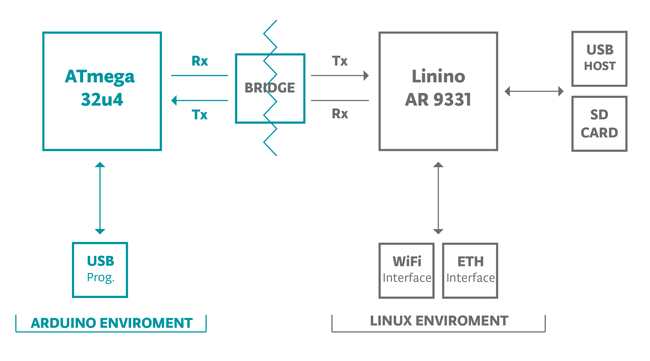
\includegraphics[width=0.8\textwidth]{/yun_processor.png}
\caption{Entornos del Arduino-Yún~\cite{Arduino-Yun}}
\label{fig:yun_processor}
\end{figure}

\begin{figure}[!h]
\centering
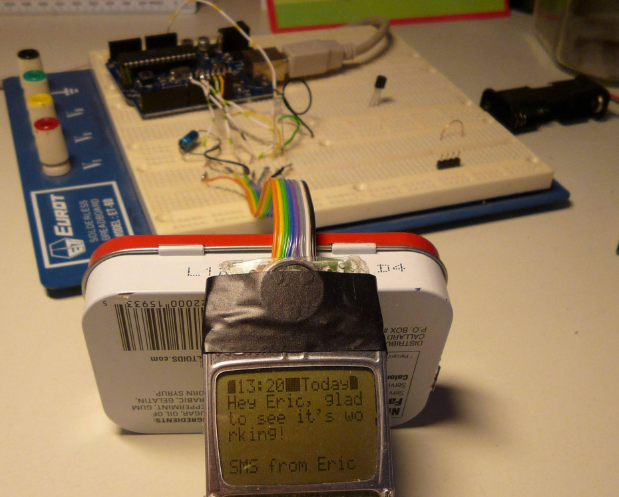
\includegraphics[width=0.8\textwidth]{/peeble_prot.png}
\caption{Prototipo Peeble~\cite{Peeble}}
\label{fig:peeble_prot}
\end{figure}

A día de hoy encontramos cientos de empresas que emplean Arduino para el desarrollo de sus productos, no solo en la fase de prototipado, también en la de producción y comercialización de un producto final. Un ejemplo de estas compañías es Pebble, que desarrolló un prototipo de reloj inteligente con una placa Arduino y una vieja pantalla LCD de un teléfono Nokia (ver Figura~\ref{fig:peeble_prot}) y más tarde recurrió a Kickstarter en busca de \$10000 de financiación para la producción y venta de unas pocas unidades y llegaron a recaudar más de \$10 000 000 (ver Figura ~\ref{fig:peeble_kickstarter}).

\begin{figure}[hp]
\centering
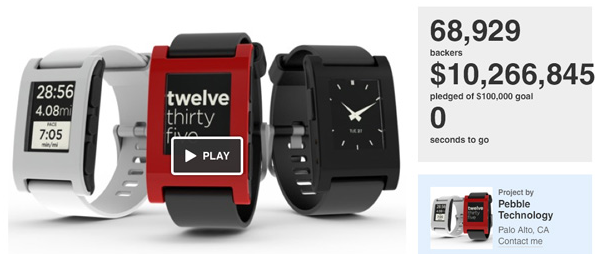
\includegraphics[width=0.8\textwidth]{/peeble_kickstarter.png}
\caption{Proyecto Peeble: Recaudación en Kickstarter~\cite{Peeble}}
\label{fig:peeble_kickstarter}
\end{figure}

\subsection{Raspberry Pi}

Desde su lanzamiento en febrero del año 2012, por parte de la Fundación Raspberry Pi, hasta la actualidad se han llegado a vender mas de 10000000 de placas \cite{NacionRS}. La familia Raspberry ha crecido en modelos, desarrolladores, revistas dedicadas y sector comercial. Sin duda alguna es uno de los candidatos más importantes a tener en cuenta en el desarrollo y evolución del sector \acf{IoT} (ver Figura~\ref{fig:iot_raspeberry}).

\begin{figure}[!h]
\centering
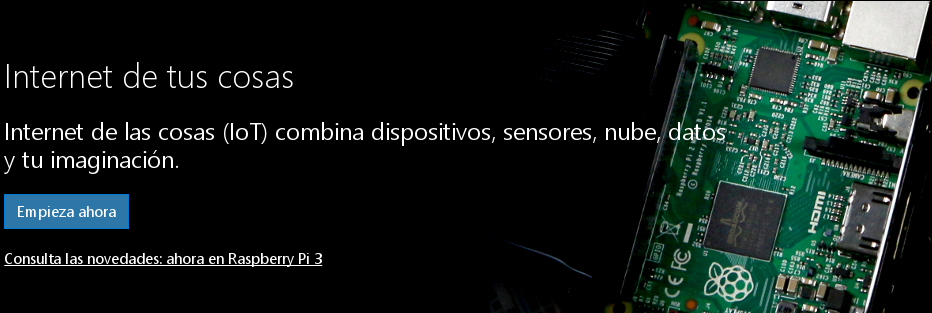
\includegraphics[width=0.95\textwidth]{/iot_raspberry.png}
\caption{Microsoft y Raspberry: la herramienta perfecta para IoT \cite{RaspberryPiIoT}}
\label{fig:iot_raspeberry}
\end{figure}

La  Raspberry  Pi es una familia de micro  ordenadores  de  altas prestaciones  que  no solo  tiene  un  rendimiento increíble, también ofrece un sinfín de posibilidades a un precio sumamente competitivo (ver Figura~\ref{fig:raspeberry_price}) que puede oscilar desde los 18,30\euro{}  para el modelo A+ hasta los 32,99\euro{}  que cuesta la nueva Raspberry Pi  Modelo B. El hecho de  tener unas dimensiones  y un  consumo muy reducido  hacen de ella el equipo  ideal en cuanto a espacio y consumo (\hyperref[chap:anexo5]{ver Anexo~\ref{chap:anexo5}}), pudiendo  ubicarse el hardware  en cualquier armario o cuarto técnico sin necesidad de tener un mobiliario grande o costoso (racks,  mesas, etc.). 

\begin{figure}[!h]
\centering
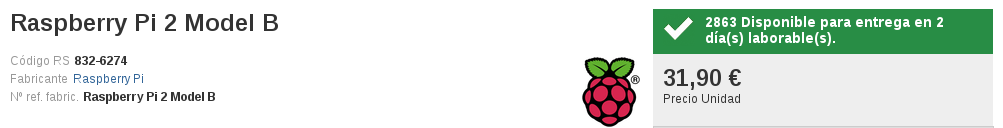
\includegraphics[width=0.8\textwidth]{/raspberry_price.png}
\caption{Precio de venta Raspberry Pi 2 Modelo B en RS Componentes~\cite{RSCompPi2}}
\label{fig:raspeberry_price}
\end{figure}

No es de extrañar que a día de hoy la Raspberry Pi se use en entornos profesionales con la finalidad de soportar servicios que puedan ser necesarios para las empresas, sobre todo las pequeñas, como un servidor web o un servidor de correo electrónico. Un ejemplo de los dos casos anteriores son:

\begin{itemize}
\item \textbf{RPi Nginx Webserver}\footnote{\url{http://elinux.org/RPi_Nginx_Webserver}}: Un servidor web más adecuado y eficiente para entornos con recursos limitados que cuenta con el apoyo de PHP\footnote{\url{http://www.php.net/manual/es/}} y MySQL\footnote{\url{http://dev.mysql.com/doc/}}. Instalable ya sea desde el paquete Debian oficial o desde el repositorio propio de Raspbian\footnote{\url{https://www.raspberrypi.org/downloads/raspbian/}}.
\item \textbf{RPi webserver\footnote{\url{http://elinux.org/RPi_webserver}}}: Un servidor web, aún más ligero que Nginx basado en Lighttpd\footnote{\url{https://www.lighttpd.net/}}.

\item \textbf{Raspberry Pi E-mail Server}: No es un programa específico, sino un conjunto de aplicaciones que en su conjunto dan un servicio integral y de calidad al usuario. Postfix\footnote{\url{http://www.postfix.org/}} para enviar y recibir correo electrónico mediante \acf{SMTP}, SquirrelMail\footnote{\url{https://squirrelmail.org/}} para comprobar el correo electrónico desde cualquier navegador y en cualquier lugar y Spamassassin\footnote{\url{http://spamassassin.apache.org/}} para auditar el correo electrónico y decidir si  es o no correo no deseado.
\end{itemize}

\lstinputlisting[label = {code:nginx_deb}, caption = {Instalación Nginx mediante el paquete de Debian Nginx.org}, style = customconsole]{code/nginx.console}

\lstinputlisting[label = {code:nginx_raspbian}, caption = {Instalación Nginx desde el repositorio de Raspbian}, style = customconsole]{code/nginx_raspbian.console}

\section{Soluciones comerciales}

Las soluciones comerciales de \acs{SES} que podemos encontrar en el mercado actualmente son tan variopintas como puntos de vistas o enfoques tengan los fabricantes. En el sector de la seguridad las líneas entre sistema de seguridad, domótica, y recientemente, «aplicación en la nube» se desdibujan con facilidad. Por este motivo resulta muchas veces difícil categorizar un sistema o plataforma y poder discernir claramente,  si es domótica que integra seguridad, como Wattio\footnote{\url{https://wattio.com/es/}} o si por el contrario es una plataforma integradora de subsistemas de seguridad, como Desico\footnote{\url{http://www.desico.com/es/Vigiplus-Arquitectura-CentralizadoCluster}}, que también da soporte a elementos de tipo \acf{PLC}.

Esta situación no es más que el resultado del interés de los fabricantes de ofrecer un producto especializado en una rama concreta de la seguridad como pueda ser el control de accesos o la intrusión, sin la necesidad de abandonar otras funcionalidades que no pertenecen específicamente a la rama en cuestión pero que aportan un valor añadido.

A continuación se muestran algunas soluciones actuales agrupadas según su especialidad.

\subsection{Plataforma única y unificada centrada en la seguridad}

Según la naturaleza de ciertas infraestructuras y su funcionalidad, nos podemos encontrar con algunas de carácter crítico o de alto riesgo como puedan ser las centrales nucleares, bases militares, aeropuertos, etc. No es de extrañar que en estas instalaciones se doten de una amplia variedad de sistemas y sensores que generan una gran cantidad de información en el centro de control o en la \acs{CRA} a la que están conectados dichos sistemas y que debe ser tratada manualmente por los operadores(ver Figura~\ref{fig:sin_psim}).

\begin{figure}[h]
\centering
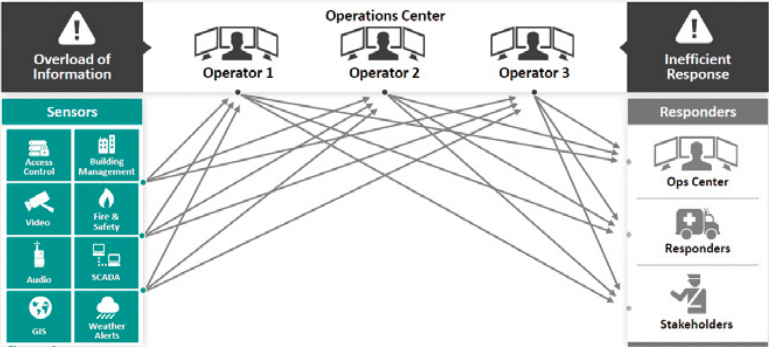
\includegraphics[width=0.9\textwidth]{/sin_psim.png}
\caption{Situación estándar de un centro de control sin un software \acs{PSIM} ~\cite{PSIM_EnriqueSoto}}
\label{fig:sin_psim}
\end{figure}

Es importante, por tanto, disponer de una solución que permita unificar en una única plataforma todos los sistemas de seguridad de una organización (\acs{CCTV}, intrusión, control de accesos, control y extinción de incendios y ciberseguridad), los sistemas de comunicaciones y de gestión de edificios (climatización , ascensores, iluminación), así como diversas fuentes de datos externas como puedan ser información del tráfico o del tiempo.

Es aquí donde entran en juegos los sistemas \acf{PSIM}, constituyendo la columna vertebral de la solución y aportando la interfaz para representar y gestionar toda la información y subsistemas comentados anteriormente en una única plataforma.

\begin{figure}[h]
\centering
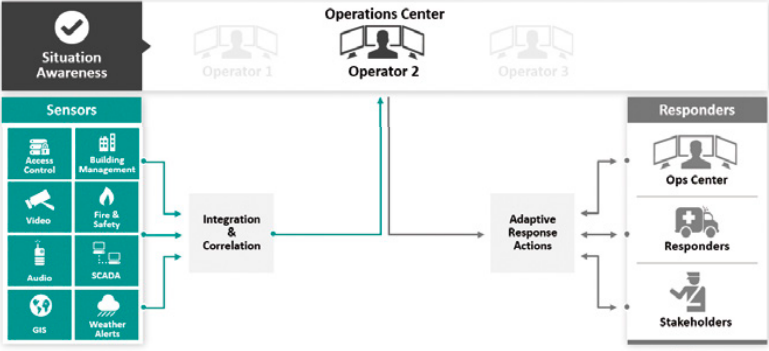
\includegraphics[width=0.9\textwidth]{/con_psim.png}
\caption{Gestión mediante software \acs{PSIM}~\cite{PSIM_EnriqueSoto}}
\label{fig:con_psim}
\end{figure}

Según el criterio de Enrique Soto, Director Técnico del Área Seguridad del \textbf{Grupo Álava}\footnote{\url{http://www.alava-ing.es/ingenieros/}}, un \acs{PSIM} debe proporcionar al menos cinco facilidades clave.

\begin{quote}
{\itshape
\begin{enumerate}
\item \textbf{Recolección}: Mediante un software independiente de los dispositivos que recoja datos de distintos elementos o sistemas de seguridad.
\item \textbf{Análisis}: El sistema debe analizar y correlacionar datos, eventos y alarmas para identificar claramente la situación real y establecer los niveles de prioridad adecuados.
\item \textbf{Verificación}: El software \acs{PSIM} tiene que mostrar la información relevante de forma rápida y amigable a los operadores para que puedan verificar la situación real con precisión.
\item \textbf{Resolución}: El sistema debe proporcionar procedimientos operativos con instrucciones paso a paso, basados en buenas prácticas y políticas de la organización y que permitan resolver, de forma eficaz, las diversas situaciones que se puedan presentar.
\item \textbf{Informes}: el software \acs{PSIM}, además de analizar la información y registrar los pasos ejecutados debe generar informes de conformidad que faciliten la depuración, la mejora de procedimientos, la formación, y en caso necesario, un análisis de profundidad.
\end{enumerate}
}
\nopagebreak
\par\nointerlineskip\noindent\hfill Fuente~\cite{PSIM_EnriqueSoto}
\end{quote}

Veamos a continuación algunos ejemplos de soluciones comerciales y cuáles son sus principales ventajas competitivas según sus fabricantes.

\subsubsection{Agora}

Agora es un \acs{PSIM} especializado en la monitorización de alarmas, que integra todo el equipamiento necesario y optimiza las operaciones de:
\begin{quote}
\begin{itemize}
\item \textbf{Vídeo Verificación}: Muestra al operador un conjunto de instrucciones previamente configuradas por el instalador que le permite discernir una falsa alarma o falso positivo de un alarma real.
\item \textbf{Rondas de Vigilancia Remota}: Evita la necesidad de tener a un vigilante que realice la ronda localmente, gracias a que presenta al operador del centro de control imágenes de una serie de lugares junto con información relevante de los mismos y del estado de los sistemas. Un punto muy fuerte es que el operador a medida que hace la ronda debe ir respondiendo preguntas al respecto y sobre lo que observa, lo que consigue que la ronda se haga prestando la máxima atención y que quede constancia verificada de que el operador estuvo supervisando la operación.
\item \textbf{Gestión de Entrada/Salida}: Este módulo permite al operador remoto conceder o denegar el acceso al recinto supervisado sin la necesidad de tener instalado algún sistema de control de accesos. El operador hace una verificación por vídeo y audio y desactiva las particiones necesarias del sistema de intrusión remotamente, dejando constancia del acceso y del porqué de la desactivación del sistema.
\item \textbf{Control de Acceso Supervisado}: El operador supervisa todas las alertas generadas por el sistema de control de accesos, dejando un registro detallado de por qué se ha producido la incidencia y solventándola si es posible.
\item \textbf{Supervisión \textit{Lonerworker}}: El operador remoto puede supervisar la integridad física de un trabajador o de un miembro del equipo de seguridad desplazado a la instalación, mediante un protocolo de contacto en caso de ausencia de noticias del mismo o por la pulsación de algún botón de emergencia portátil con mecanismo de geolocalización.
\item \textbf{Escolta \acs{VIP}}: El operador remoto se encontrará en contacto y seguirá gracias a un GPS los movimientos de la persona escoltada.
\item \textbf{Prueba de Servicio}: La plataforma permite a su administrador consultar y auditar todas las acciones, incluso el vídeo y audio consultado por el operador del sistema y verificar si ha cumplido con el procedimiento operativo establecido, o no.
\item \textbf{Tiempo de Respuesta}: La plataforma mejora drásticamente los tiempos de respuesta ante incidencias debido a que los operadores reciben todas las alarmas en curso, ordenadas por prioridad y correlacionadas por sitios. Cuando un operador comienza el tratamiento de una alarma, este se encuentra guiado durante todo el proceso gracias a fáciles instrucciones que le indican como tratar la incidencia.
\end{itemize}
\par\nointerlineskip\noindent\hfill Fuente~\cite{AGORA_PSIM}
\end{quote}

\subsection{Edificios y casas inteligentes}

Aunque pueda parecer que hablamos de domótica, los sistemas que se comentan en esta sección van un paso más allá y se podría decir que se engloban en la categoría de softwares \acs{PSIM} pero se centran en ofrecer ciertas ventajas competitivas centradas en la gestión integral de los sistemas de los edificios y hogares. 

\subsubsection{Desigo CC}

El pasado 30 de marzo del 2016, la compañía Siemens\footnote{\url{http://www.buildingtechnologies.siemens.com/bt/sp/en/security-products/pages/security-products.aspx}} presentó su sistema más innovador hasta la fecha en la gestión de edificios inteligentes.

\textbf{Desigo CC}\footnote{\url{http://www.buildingtechnologies.siemens.com/bt/global/en/building-solutions/desigo-cc/pages/desigo-cc.aspx}}, es la primera plataforma con la que cuenta la multinacional, capaz de gestionar todos los sistemas y tecnologías de los edificios con importantes ahorros en energía y con una integración total de los sistemas de seguridad existentes~(ver Figura~\ref{fig:desigo}). Esta plataforma centraliza y gestiona desde un único puesto de control todas las disciplinas del edificio: climatización, ventilación, protección contra incendios, control de accesos, iluminación, control de persianas, videovigilancia e intrusión~\cite{DESIGO}. 

Además del ahorro de hasta el 20\% que podemos obtener de la gestión inteligente de la iluminación, control de persianas y climatización, esta plataforma ofrece la ventaja de ser capaz de responder a las necesidades de los operadores desde cualquier lugar y en cualquier momento. Los gestores de la plataforma pueden acceder remotamente ya sea desde una tablet o un \textit{smartphone} y acceder a todas las funcionalidades que les ofrece el sistema, pudiendo monitorizar el rendimiento energético y dar respuesta inmediata a las alarmas recibidas.

\begin{figure}[!h]
\centering
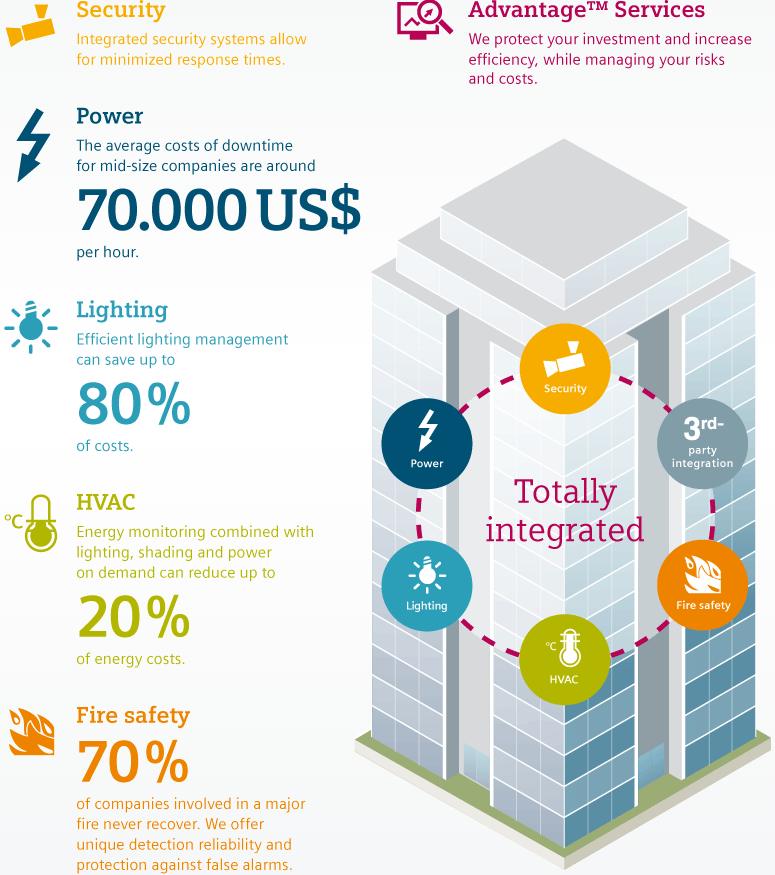
\includegraphics[width=0.8\textwidth]{/desigo.png}
\caption{Gestión de edificios con Desigo CC~\cite{Desigo_Img}}
\label{fig:desigo}
\end{figure}

\subsubsection{Risco Group}

\textbf{Risco Group}\footnote{\url{http://www.riscogroup.com/spain/}} es un fabricante de productos de seguridad para toda clase de instalaciones y un ejemplo de la introducción de tecnología de bajo coste y altas prestaciones. Entre las soluciones comerciales más interesantes que ofrece esta compañía se encuentan:

\begin{itemize}
\item \textbf{Smart Home}\footnote{\url{http://www.riscogroup.com/spain/content/smart-home-de-risco}}: Es una solución integral de automatización profesional para el hogar. Además de permitir al usuario controlar la iluminación, climatización, cerraduras inteligentes y otros dispositivos y sistemas del hogar desde su \textit{smartphone} a través de la aplicación iRISCO\footnote{\url{https://play.google.com/store/apps/details?id=com.homeguard&hl=es}}, también permite armar y desarmar particiones y realizar vídeo verificación ante la recepción de nuevos eventos~\cite{RiscoGroupSmartHome}.

Es preciso hacer hincapié en cómo el propio fabricante define su producto y hacia quién va orientada la definición. 

\begin{quote}
«\textit{Smart Home de Risco Group es una oportunidad puntera para los instaladores que buscan aumentar su potencial de negocios con las soluciones más avanzadas y completas de automatización para el hogar}».
\par\nointerlineskip\noindent\hfill Fuente~\cite{RiscoGroupSmartHome}
\end{quote}

Como vemos en el mercado de la seguridad, es casi más importante dirigir un producto al gusto del sector instalador, que es el que provee a los fabricantes de una cuota importante de ventas que hacia el usuario final.

\item \textbf{ProSYS$^{TM}$ Plus}\footnote{\url{http://www.riscogroup.com/spain/products/solution/51027}}: «\textit{ combina las mejores tecnologías de RISCO Group, incluyendo la aplicación para dispositivos móviles iRISCO para controlar remotamente el sistema, cámaras IP integradas para una vídeo verificación en tiempo real en alta resolución y ver lo que sucede, así como una amplia gama de detectores profesionales comerciales e industriales.  ProSYS ™ Plus ha sido diseñada para trabajar con las últimas tecnologías de comunicación disponibles - incluyendo IP “multi-socket”, 3G\footnote{\url{https://en.wikipedia.org/wiki/3G}} / 4G\footnote{\url{https://en.wikipedia.org/wiki/4G}} y WiFi\footnote{\url{https://es.wikipedia.org/wiki/Wifi}}}»
\end{itemize}

\subsection{\acf{CCTV}}

Como no podía ser de otra manera, una vez comentadas algunas plataformas y sistemas de seguridad toca abordar la videovigilancia y más cercanamente a lo que toca este proyecto, la videovigilancia de bajo coste (cámaras y plataformas de videograbación).

Cuando hablamos de los gigantes del \acs{CCTV} no podemos olvidar mencionar a fabricantes de cámaras como Axis\footnote{\url{http://www.axis.com/es/es/}} y Pelco\footnote{\url{https://www.pelco.com/}}, o de plataformas de viodeograbación avanzadas, Milestone\footnote{\url{https://www.milestonesys.com/}} y Geutebrück\footnote{\url{http://www.ffvideosistemas.com/}}, todas ellas grandes compañías con un capital cuantioso invertido en \acs{I+D} y con nicho de mercado asentado en España con más de 10 años de antigüedad. Sin embargo son las compañías como Dahua\footnote{\url{http://www1.dahuasecurity.com/es/}} y Hikvision\footnote{\url{http://www.hikvision.com/europe/index.html}} las que han logrado dinamizar el mercado actual poniendo a disposición de cualquiera, con unos pocos cientos de euros (ver Figura~\ref{fig:hik}), la tecnología que antes estaba reservada a corporaciones con grandes inversiones en seguridad.

\begin{figure}[!h]
\centering
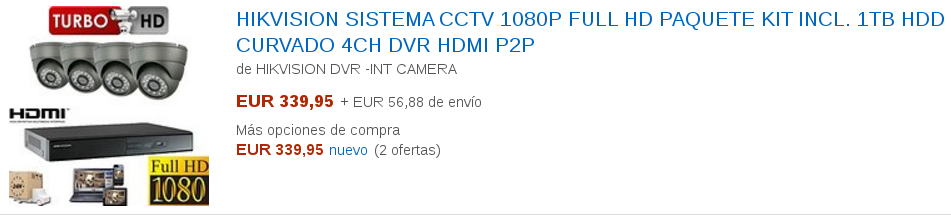
\includegraphics[width=1\textwidth]{/hik.png}
\caption{Búsqueda en Amazon de productos Hikvision~\cite{Hik_Amz}}
\label{fig:hik}
\end{figure}

Veamos a continuación cuales son sus estrategias de negocio y como prevén la evolución del sector en los próximos años.

\pagebreak

\subsubsection{Dahua}

\begin{quote}
{\itshape
\textbf{¿Qué estrategia de negocio y proyectos va a llevar a cabo Dahua en 2016?}

\textit{Para expandir nuestro negocio pensamos en dos importantes puntos, como son expansión y protección. Para alcanzar el primero nos centraremos en producto y mercado. Para productos, no nos conformaremos solo con CCTV, también nos focalizaremos en \acs{VPD}, \acs{TV WALL}, alarmas, cámaras térmicas, etc. Respecto a mercados, empezaremos por \acs{IT}, mercado electrónico. En mercado vertical daremos soluciones de soporte a los mejores proyectos. En lo que respecta a protección, Dahua
siempre ayuda a sus clientes. Ahora el mercado en España está bajo una gran presión, muchos competidores con otras marcas. Dahua ayudará no solo en precio y apoyo técnico, sino también
en la expansión de productos, como VDP. Además de innovación, también prestaremos atención a la post venta, para dar el mejor servicio}.

\textbf{¿Dahua puede predecir la próxima generación o innovación en CCTV? Respecto a este cambio,
¿qué puede hacer Dahua para mantener esa posición?}

En los próximos años, el mercado de \acs{CCTV} seguirá dividiéndose en dos partes:
el mercado analógico y el de IP\footnote{\url{https://en.wikipedia.org/wiki/IP_camera}}. Respecto al analógico, debido al vídeo y audio en tiempo real y al control de la señal en un solo cable, los precios competitivos, las características, etc, los productos \acs{HD} analógicos ocuparán
una determinada cuota de mercado y las resoluciones más altas como la 4MP e incluso la 4K\footnote{\url{https://en.wikipedia.org/wiki/4K_resolution}}, serán requeridas. En relación al mercado IP, la resolución más alta, las cámaras de análisis de vídeo front-end y la tecnología H265\footnote{\url{https://es.wikipedia.org/wiki/H.265}} serán tendencia. Dahua lanzará la más alta resolución \acs{HDCVI}\footnote{\url{https://en.wikipedia.org/wiki/Dahua_Technology}} y las cámaras IP H265
con más alta resolución para mantener el liderazgo del mercado \acs{CCTV}.
}

\par\nointerlineskip\noindent\hfill Entrevista Dahua Iberia~\cite{DahuaIberia}
\end{quote}

\subsubsection{Hikvision}

Hikvision es actualmente uno de los principales proveedores a nivel mundial de productos \acs{CCTV}. Con una inversión anual en \acs{I+D} del 8\% de sus ingresos anuales, 5400 ingenieros en plantilla, entre los cuales más de 2000 ingenieros son de software, ha logrado ofrecer no solo productos de calidad a un precio que hasta ahora parecían imposibles, sino que ha aportado a ese producto los medios software necesarios para su correcta y óptima explotación~\cite{HikEurope}.

Con 30 sucursales en China y más de 18 filiales regionales por todo el mundo, Hikvision ha llevado a cabo en los últimos años una intensa carrera por ser el líder a nivel mundial de los productos \acs{CCTV} de bajo coste (no de baja calidad).

En una entrevista a David Lorente, Asistente de Marketing de Hikvision España, este definió muy claramente la visión de la compañía respecto a lo que debe ser una empresa de seguridad y sus \textit{partners}.


«\textit{Contar con los partners adecuados es de vital importancia para cualquier negocio,el valor de un partner tecnológico se mide por su capacidad de generar ventaja competitiva, por su innovación, así como por su actitud y el poder de transmitir determinación, entusiasmo y motivaciones siempre
nuevas. Una empresa creada para la seguridad, que conoce el mercado e invierte en tecnología y sus aplicaciones, dedicada a los profesionales, que hace que la seguridad sea el único foco de su
negocio es un valor esencial a la hora de elegir un partner en el sector de la seguridad}»~\cite{HikSpain}.


% Debido a su continuo uso, se muestra entre paréntesis la combinación del modo
% \texttt{auctex} de GNU Emacs para incluir el comando \LaTeX{} correspondiente.

% \begin{itemize}
% \item Normal.
% \item \textbf{Negrita} (C-c-f-b).
% \item \textit{Itálica} (C-c-f-i).
% \item \emph{Enfatizada} (C-c-f-e). Fíjate que el estilo que se obtiene al
%   enfatizar depende del estilo del texto en el que se incluya: \textit{texto en
%     itálica y \emph{enfatizado} en medio}.
% \item \texttt{Monoespaciada} (C-c-f-t)
% \end{itemize}

% Otros de menos uso:

% \begin{itemize}
% \item \textsc{Versalita} (C-c-f-c).
% \item \textsf{Serifa}, es decir, sin remates o paloseco (C-c-f-f).
% \item \textrm{Romana} (C-c-f-r).
% \end{itemize}


% \section{Viñetas y enumerados}

% En \LaTeX{} hay tres tipos básicos de viñetas:

% \begin{itemize}
% \item itemize.
% \item enumerate.
% \item description.
% \end{itemize}


% Es posible hacer viñetas (como la siguiente) cambiando márgenes u otras
% propiedades gracias al paquete
% \href{http://mirror.ctan.org/macros/latex/contrib/enumitem/enumitem.pdf}{\emph{enumitem}}
% (ya incluido en \esitfg).

% \begin{itemize}[noitemsep, label=$\triangleright$]
% \item esto es
% \item una pequeña
% \item muestra
% \end{itemize}

% El paquete \emph{enumitem} ofrece muchas otras posibilidades para personalizar
% las viñetas (individual o globalmente) o crear nuevas.


% \section{Figuras}

% Las figuras se referencian así (ver Figura~\ref{fig:informatica}). Recuerda que
% no tienen porqué aparecer en el lugar donde se ponen (mira un libro de
% verdad). \LaTeX{} las colocará donde mejor queden, No te empeñes en
% contradecirle, él sabe mucho de tipografía.

% \begin{figure}[!h]
% \begin{center}
% \includegraphics[width=0.2\textwidth]{/informatica.pdf}
% \caption{Escudo oficial de informática}
% \label{fig:informatica}
% \end{center}
% \end{figure}

% Por cierto, los títulos de tablas, figuras y otro elementos flotantes (los
% \texttt{caption}) no deben acabar en punto~\cite{sousa}.


% \section{Cuadros}
% \label{sec:uncuadro}

% Se denominan «tablas» cuando contienen datos con relaciones numéricas. El
% término genérico (que debe usarse cuando en los demás casos) es
% «cuadro»~\cite{sousa}. Si las columnas están bien alineadas, las líneas
% verticales estorban más que ayudan (no las pongas). Los cuadros se referencian
% de este modo (ver Cuadro~\ref{tab:rpc-semantics}).

% \begin{table}[hp]
%   \centering
%   {\small
%   


\begin{tabular}{p{.2\textwidth}p{.2\textwidth}p{.2\textwidth}p{.2\textwidth}}
  \tabheadformat
  \tabhead{Tipo de fallo}   &
  \tabhead{Sin fallos}      &
  \tabhead{Mensaje perdido} &
  \tabhead{Servidor caído}  \\
\hline
\textit{Maybe}         & Ejecuta:   1 & Ejecuta: 0/1        & Ejecuta: 0/1 \\
                       & Resultado: 1 & Resultado: 0        & Resultado: 0 \\
\hline
\textit{Al-least-once} & Ejecuta:   1 & Ejecuta:   $\geq$ 1 & Ejecuta:   $\geq$ 0 \\
                       & Resultado: 1 & Resultado: $\geq$ 1 & Resultado: $\geq$ 0 \\
\hline
\textit{At-most-once}  & Ejecuta:   1 & Ejecuta:   1        & Ejecuta: 0/1 \\
                       & Resultado: 1 & Resultado: 1        & Resultado: 0 \\
\hline
\textit{Exactly-once}  & Ejecuta:   1 & Ejecuta:   1        & Ejecuta:   1 \\
                       & Resultado: 1 & Resultado: 1        & Resultado: 1 \\
\hline
\end{tabular}


% Local variables:
%   coding: utf-8
%   ispell-local-dictionary: "castellano8"
%   TeX-master: "main.tex"
% End:

%   }
%   \caption[Semánticas de \acs{RPC} en presencia de distintos fallos]
%   {Semánticas de \acs{RPC} en presencia de distintos fallos
%     (\textsc{Puder}~\cite{puder05:_distr_system_archit})}
%   \label{tab:rpc-semantics}
% \end{table}


% \section{Listados de código}
% \label{sec:listado}

% Puedes referenciar un listado así (ver Listado~\ref{code:hello}). Éste es un
% listado flotante, pero también pueden ser «no flotantes» quitando el parámetro
% \texttt{float} (mira el fuente de este documento o la referencia del paquete
% \href{http://www.ctan.org/get/macros/latex/contrib/listings/listings.pdf}{«listings»}).

% \begin{listing}[
%   float=ht,
%   language = C,
%   caption  = {«Hola mundo» en C},
%   label    = code:hello]
% #include <stdio.h>
% int main(int argc, char *argv[]) {
%     puts("Hola mundo\n");
% }
% \end{listing}

% \noindent
% Puedes incluir un fichero de código fuente (o un fragmento) con \texttt{lstinputlisting}:

% \lstinputlisting[language=C, firstline=3, texcl]{code/hello.c}

% \noindent
% Y también existe un comando \texttt{console} para representar ejecución de
% comandos:

% \begin{console}
% $ uname --operating-system
% GNU/Linux
% \end{console} %$

% Puedes modificar el estilo por defecto para tus listados añadiendo un comando
% \texcmd{lstset} en tu \texttt{custom.sty}. El código \LaTeX{} del listado
% \ref{code:custom-listings} añade un fondo gris claro y una línea en el margen
% izquierdo.

% \begin{listing}[
%   float=h!,
%   caption  = {Personalizando los listados de código},
%   label    = code:custom-listings]
% \lstset{%
%   backgroundcolor = \color{gray95},
%   rulesepcolor    = \color{black},
% }
% \end{listing}

% En cualquier caso, si lo necesitas siempre es mejor que redefinas los comandos y entornos
% existentes o crees entornos nuevos, en lugar de añadir los mismos cambios en
% muchas partes del documento.



% \section{Citas y referencias cruzadas}

% Puedes ver aquí una cita~\cite{design_patterns} y una referencia a la segunda sección
% (véase \S\,\ref{sec:uncuadro}). Para hacer referencias debes definir etiquetas en el punto
% que quieras referenciar (normalmente justo debajo). Es útil que los nombres de las
% etiquetas (comando label) tengan los siguientes prefijos (incluyendo los dos puntos ``:''
% del final):

% \begin{description}
% \item[chap:] para los capítulos. Ej: ``\texttt{chap:objetivos}''.
% \item[sec:] para secciones, subsecciones, etc.
% \item[fig:] para las figuras.
% \item[tab:] para las tablas.
% \item[code:] para los listados de código.
% \end{description}

% Si estás viendo la versión PDF de este documento puedes pinchar la cita o el número de
% sección. Son hiper-enlaces que llevan al elemento correspondiente. Todos los elementos que
% hacen referencia a otra cosa (figuras, tablas, listados, secciones, capítulos, citas,
% páginas web, etc.) son «pinchables» gracias al paquete
% \href{http://latex.tugraz.at/_media/docs/hyperref.pdf}{\emph{hyperref}}.

% Para citar páginas web usa el comando \texttt{url} como en: \url{http://www.uclm.es}

% \section{Páginas}
% \label{sec:paginas}

% La normativa aconseja imprimir el documento a doble cara, pero si el número de
% páginas es bajo puede imprimirse a una cara. Como eso es bastante subjetivo, mi
% consejo es que ronde las 100 \textbf{hojas}. Una hoja impresa a doble cara
% contiene 2 páginas, a una cara contiene una. Es decir, si el documento tiene más
% de 200 páginas imprímelo a doble cara, si tiene menos imprímelo a una.

% Por defecto, \esitfg{} imprime a una cara (oneside), si quieres imprimir a doble cara,
% escribe en el preámbulo:

% \begin{listing}
%   \documentclass[twoside]{esi-tfg}
% \end{listing}

% Esto es importante porque a doble cara los márgenes son simétricos y a una cara
% no. Si llevas el TFG a la copistería y pides que te lo impriman de modo
% diferente al generado, quedará mal ¡Cuidado!

% Tal como indica la normativa, los capítulos siempre empiezan en la página
% derecha, la impar cuando se usa doble cara.


% Local Variables:
%  coding: utf-8
%  mode: latex
%  mode: flyspell
%  ispell-local-dictionary: "castellano8"
% End:
